\documentclass[12pt]{jarticle}
\usepackage{TUSIReport}
\usepackage{otf}
\usepackage[dvipdfmx]{graphicx}
\usepackage[dvipdfmx]{color}
\usepackage{amsmath}
\usepackage{amssymb}
\usepackage{color}
\usepackage{hhline}
\usepackage{fancybox,ascmac}
\usepackage{multirow}
\usepackage{url}
\usepackage{bm}
\usepackage{listings,jlisting}

\begin{document}
%%%%%%%%%%%%%%%%%%%%%%%%%%%%%%%%%%%%%%%%%%%%%%%%%%%%%%%%%%%%%%
% 表紙を出力する場合は,\提出者と\共同実験者をいれる
% \提出者{科目名}{課題名}{提出年}{提出月}{提出日}{学籍番号}{氏名}
% \共同実験者{一人目}{二人目}{..}{..}{..}{..}{..}{八人目}
%%%%%%%%%%%%%%%%%%%%%%%%%%%%%%%%%%%%%%%%%%%%%%%%%%%%%%%%%%%%%%
\提出者{情報工学実験2}{実験テーマ5 教育システム設計}{2020}{11}{16}{4619055}{辰川力駆}
\共同実験者{書かないと!}{}{}{}{}{}{}{}

%%%%%%%%%%%%%%%%%%%%%%%%%%%%%%%%%%%%%%%%%%%%%%%%%%%%%%%%%%%%%%
% 表紙を出力しない場合は,以下の「\表紙出力」をコメントアウトする
%%%%%%%%%%%%%%%%%%%%%%%%%%%%%%%%%%%%%%%%%%%%%%%%%%%%%%%%%%%%%%
\表紙出力

%%%%%%%%%%%%%%%%%%%%%%%%%%%%%%%%%%%%%%%%%%%%%%%%%%%%%%%%%%%%%%
% 以下はレポート本体である.別途 TeXファイルを作成し \input 使っても良い
%%%%%%%%%%%%%%%%%%%%%%%%%%%%%%%%%%%%%%%%%%%%%%%%%%%%%%%%%%%%%%

\section{要旨}


\section{目的}
統計モデルを用いた分析は、例えば商品の推薦や迷惑メールの削除機能など、
身近な機能を支える基本的な技術となっている。
本実験では、このような統計モデルを用いた分析に欠かせない、
パラメタの推定の方法について、
基本的な技術を習得することを目的とする。

\section{理論}
\subsection{項目反応理論:複数問の反応からの能力値推定}
複数の問題に対する正誤反応を得た場合の能力値の推定について考える。
今、
ある問題系列について正誤反応${\bf X}_j=(x_{1,j},x_{2,j},...,x_{n,j})$が
与えられたとする。
この時の能力値$\theta$の推定値を考える際には以下のような数式を考えれば良い。
\begin{eqnarray}
    \hat{\theta}&=& \mathop{\rm arg~max}\limits_{\theta} P(\theta|{\bf X}_j)\\
    &=& \mathop{\rm arg~max}\limits_{\theta} P(\theta)P({\bf X}_j|\theta)
\end{eqnarray}
ここで$P({\bf X}_j|\theta)$はある能力値$\theta$の受験者が、
それぞれの項目に${\bf X}_j$のように反応する確率である。
そのため、それぞれの項目への正誤が$\theta$のみに影響され定まるとすれば、
$P({\bf X}_j|\theta)$は以下のようにかける。
\begin{eqnarray}
    P({\bf X}_j|\theta)&=&P(x_{1,j}|\theta)\times P(x_{2,j}|\theta)\times \cdots \times P(x_{n,j}|\theta)\\
    &=& \prod_{i=1}^n P(x_{i.j}|\theta)
\end{eqnarray}
つまり、複数のサイコロを同時に投げたときと同様に同時確率とみなすことができる。
それぞれの項目への能力値$\theta$だけを媒介に独立に正誤反応していると考える。
これを局所独立仮定という。
すなわち、それぞれの項目が他の項目の答えやヒントになっていない状況である。


また、$P(x_{i,j}|\theta)$は正答の場合と
誤答の場合両方を以下のように表すことができる。
\begin{eqnarray}
    P(x_{i,j}|\theta)=P_i(\theta)^{x_{i,j}}\times (1-P_i(\theta))^{1-x_{i,j}}
\end{eqnarray}
従って、考えるべき式は以下のようになる。
\begin{eqnarray}
    \hat{\theta}&=& \mathop{\rm arg~max}\limits_{\theta} P(\theta|{\bf X}_j) \nonumber\\
    &=& \mathop{\rm arg~max}\limits_{\theta} P(\theta)\prod_{i=1}^n P(x_{i,j}|\theta) \nonumber\\
    &=& \mathop{\rm arg~max}\limits_{\theta} P(\theta)\prod_{i=1}^n (P_i(\theta)^{x_{i,j}}(1-P_i(\theta))^{1-x_{i,j}})
\end{eqnarray}
ただし、これを計算機により計算することは、
値域が$[0,1]$を取る関数を複数回かけることになり、
計算誤差が生じやすい。
そのため、実装上は、このような関数の対数関数を考える。
${\rm log}$は単調増加関数であり、
ある関数$f(x)$が$x=x_{\rm max}$で最大を取るとき、
${\rm log}(f(x))$も$x=x_{\rm max}$で最大を取る。
そのため、以下が成り立つ。
\begin{eqnarray}
    \hat{\theta}&=& \mathop{\rm arg~max}\limits_{\theta} P(\theta|{\bf X}_j)\\
    &=& \mathop{\rm arg~max}\limits_{\theta} \ln{(P(\theta|{\bf X}_j))}
\end{eqnarray}
そのため、実装上は以下を計算すれば良い。
\begin{eqnarray}
    \hat{\theta}&=& \mathop{\rm arg~max}\limits_{\theta} \Bigl\{\ln{(P(\theta))
    +\sum_{i=1}^n \Bigl(x_{i,j}\ln(P_i(\theta))+(1-x_{i,j})\ln(1-P_i(\theta))\Bigr)}\Bigr\}
\end{eqnarray}
これを対数尤度関数と呼ぶ。

\section{課題}
\subsection{課題3-1}
\begin{shadebox}
    課題2-4で描いた事後分布とその対数尤度関数を図示し、
    それぞれの最大値にどのような関係があるか示す。
\end{shadebox}

\begin{figure}[h]
    \begin{center}
        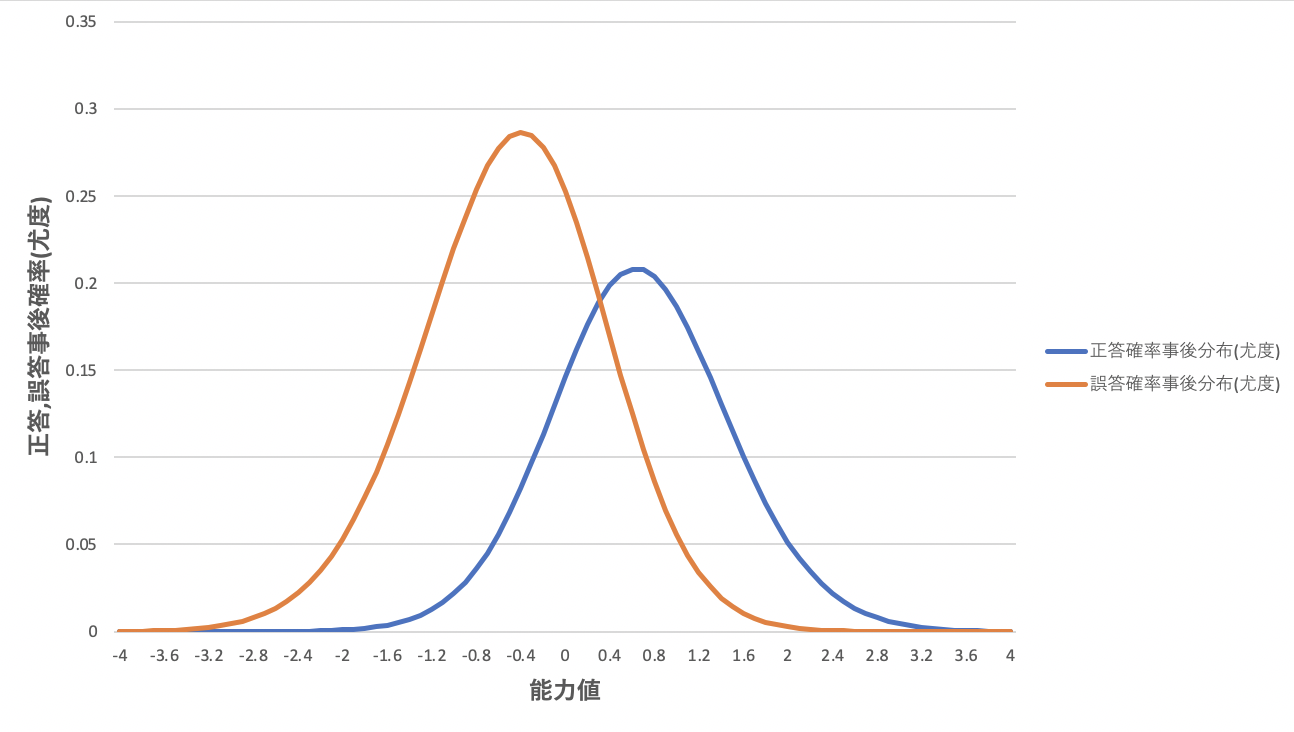
\includegraphics[scale=0.3]{kadai5_3_1.png}
    \end{center}
    \caption{Item21の正答確率事後分布と誤答確率事後分布のグラフ}
\end{figure}

\clearpage
\begin{figure}[h]
    \begin{center}
        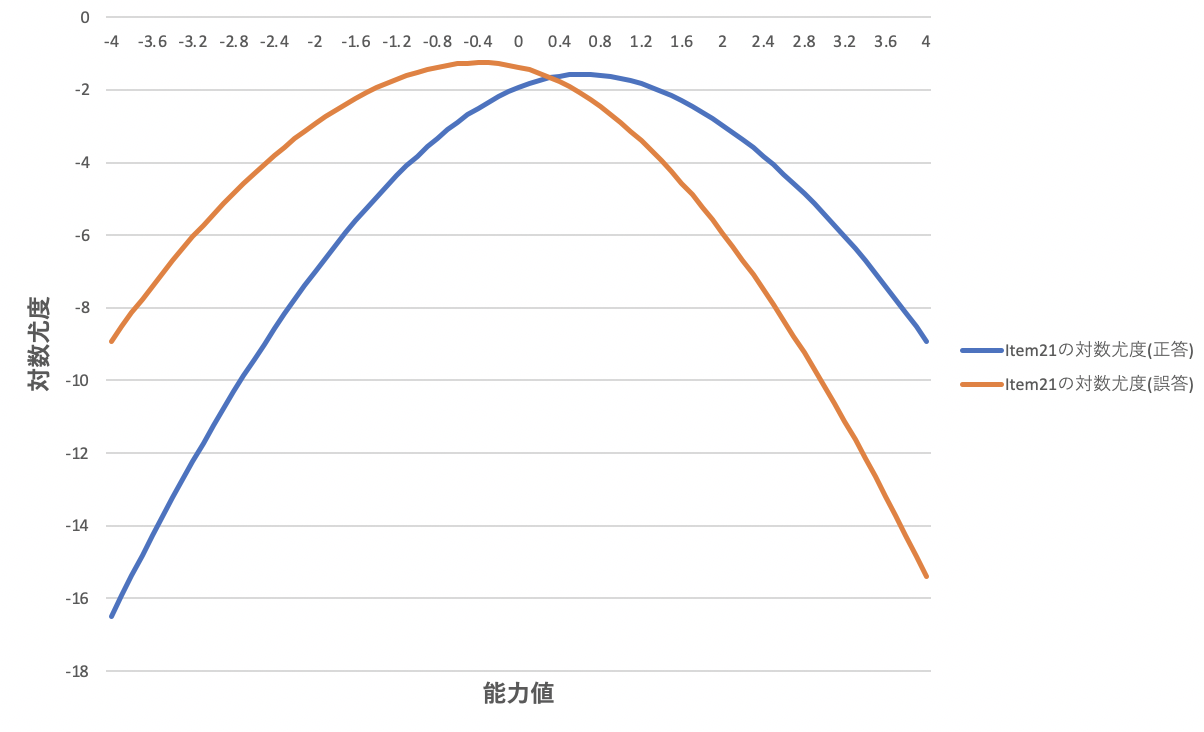
\includegraphics[scale=0.3]{kadai5_3_2.png}
    \end{center}
    \caption{Item21の正答と誤答の対数尤度グラフ}
\end{figure}

Item21の事後分布のグラフは図1のようになった。
また、対数尤度関数のグラフは図2のようになった。
尤度の値はすべて$0\sim 0.3$の間に収まっているので、
自然対数を取った対数尤度の値はすべて負の値を取っている。

対数尤度は事後分布の対数をとったものであるが、
対数関数は定義域に対して単調増加であるから、
ある関数に対し対数をとっても横軸の値に対する縦軸の値の大小関係は変化しない。
つまり、どちらのグラフも最大値を取るときの$\theta$は同じで、
正答は$\theta=0.6$で誤答は$\theta=-0.4$である。

\subsection{課題3-2}
\begin{shadebox}
    課題1-3で解いた全ての項目の反応から自分の能力値$\theta$の
    対数尤度関数の概形を示す。
\end{shadebox}

Item3,9,21,24,30,35,40,51を解き全て正答したので、
それらの正答確率の対数関数を全て足し合わせると、
グラフを求めることができる。
結果は図3ようになった。

対数関数なので、和を求めたことにより、
上記のItem21だけの対数対数尤度グラフと比べて、
最大値を取っている$\theta$の値が高くなっている。
これは全て正答したからである。

\clearpage
\begin{figure}[h]
    \begin{center}
        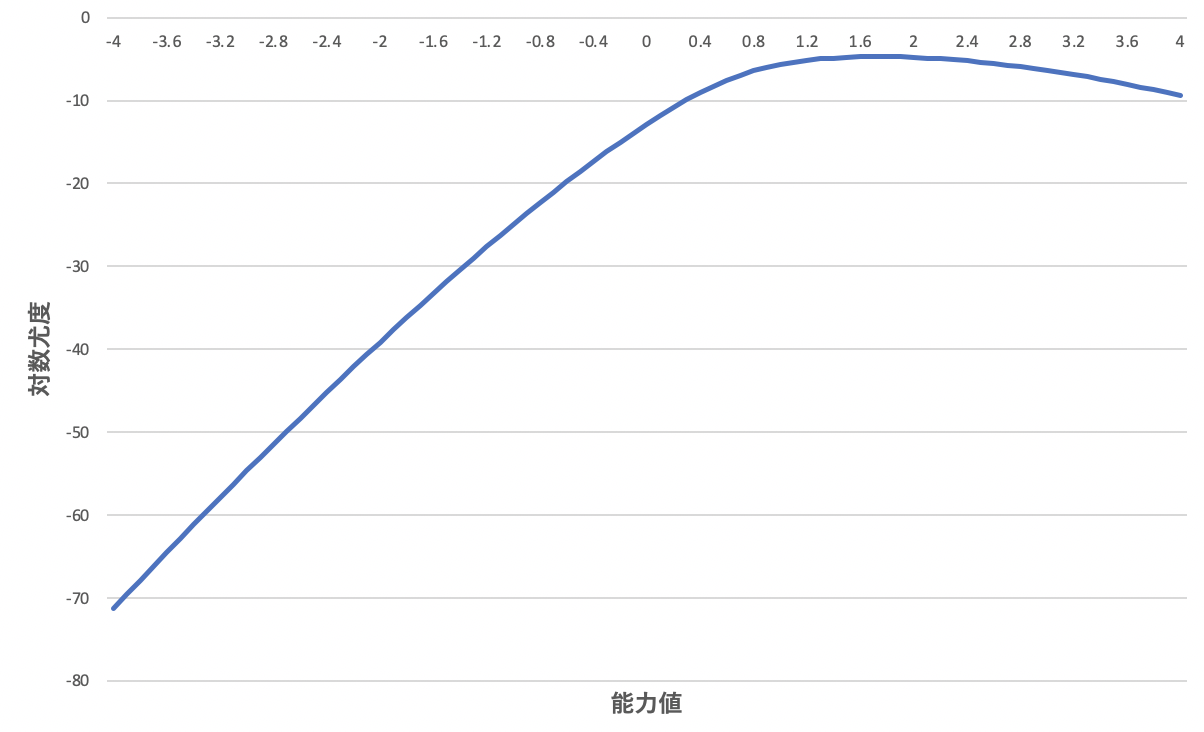
\includegraphics[scale=0.4]{kadai5_3_3.png}
    \end{center}
    \caption{全ての項目による対数尤度グラフ}
\end{figure}

\subsection{課題3-3}
\begin{shadebox}
    課題3-2で描いた対数尤度関数から能力値を推定する。
    またその時の情報量$I(\hat{\theta})$と標準誤差$se(\hat{\theta})$を求める。
\end{shadebox}

図3の対数尤度関数で最大値を取っている$\theta$の値は、
$\theta=$の時に関数は最大値をとることから自分の能力値は1.3であると推定できる.今回の情報量は各itemに関する情報量の総和であるため以下の式を用いれば良い.
\begin{eqnarray*}
    I(\hat{\theta})&=&\sum_{i=1}^{10}{I_i({\theta})}\\
    &=&\sum_{i=1}^{10}{D^2a_i^2P_i(\theta)(1-P_i(\theta))}\\
    &=&\sum_{i=1}^{10}{1.7^2a_i^2P_i(1.3)(1-P_i(1.3))}\\
    &=&0.933706345\cdots\simeq 0.93371
\end{eqnarray*}
また,標準誤差は
\begin{eqnarray*}
    se(\hat{\theta})&=&I(\hat{\theta})^{-\frac{1}{2}}\\
    &=&\frac{1}{\sqrt{0.93371}}\\
    &=&1.03489156\cdots\simeq 1.03489
\end{eqnarray*}


\subsection{課題3-4}
\begin{shadebox}
    課題1-3で解いた項目の$a_i$が全て「1」だった場合の能力値、情報量、
    標準誤差を求め、結果について考察する。
\end{shadebox}


\subsection{課題3–5}
\begin{shadebox}
    解いた項目と、能力値$\theta$の推定結果と、
    課題1-4で行なった偏差値$S$の結果を同じグループ内で共有し、
    比べた結果を考察する。
\end{shadebox}


\begin{table}[htb]
    \begin{center}
        \caption{解いた問題の特性パラメタ}
        \begin{tabular}{|c|r|r|}
            \hline
            問題 & $aパラメタ$ & $bパラメタ$ \\
            \hline
            3    & 2.87168     & 0.69892     \\
            9    & 0.42082     & 0.22627     \\
            21   & 1.03497     & 0.31148     \\
            24   & 0.71798     & 1.22817     \\
            30   & 1.20718     & 0.65633     \\
            35   & 0.72641     & 0.14052     \\
            40   & 0.31796     & 2.23511     \\
            51   & 0.51611     & 0.94029     \\
            \hline
        \end{tabular}
    \end{center}
\end{table}


\subsection{課題3c–1}
\begin{shadebox}
    課題1-3で解いた全ての項目での対数尤度関数に対して、
    ニュートン法を用いて能力値を推定する。
\end{shadebox}


\section{まとめ}



\clearpage
% 付録
\appendix
%%%%%%%%%%%%%%%%%%%%%%%%%%%%%%%%%%%%%%%%%%%%%%%%%%%%%%%%%%%%%%
\end{document}